% ================== ANNEXES ==================
\chapter*{Annexes}
\addcontentsline{toc}{chapter}{Annexes}
\chaptermark{Annexes}

\cleardoublepage
\stepcounter{chapter}
\chapter*{Annexe \thechapter{} : Matériaux de construction mécanique}
\label{annexe:materiaux_mecaniques}
\addcontentsline{toc}{section}{Annexe \thechapter{} : Matériaux de construction mécanique}
\setcounter{figure}{0}



Cette annexe regroupe les photographies des matériaux bruts (Figure \ref{fig:annexe_tube_acier}, \ref{fig:annexe_contreplaqué}, \ref{fig:annexe_pla}) choisis pour la réalisation de la structure mécanique du prototype SMART-SOJA (Figure \ref{fig:annexe_materiaux_global}).

\begin{figure}[H]
    \centering
    \begin{minipage}[b]{0.31\textwidth}
        \centering
        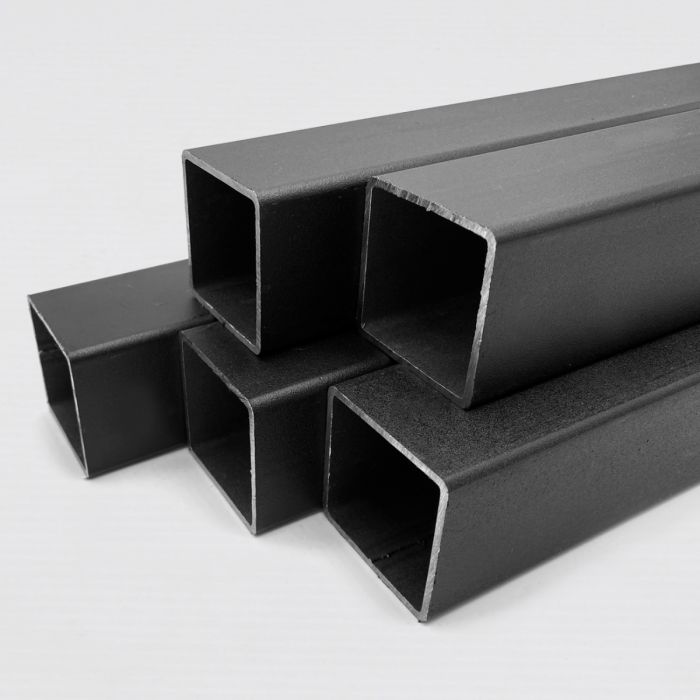
\includegraphics[width=\textwidth]{images/tube_carre_40mmx40mm.jpg}
        \caption{Profilé acier 40×40 mm}
        \label{fig:annexe_tube_acier}
    \end{minipage}
    \hfill
    \begin{minipage}[b]{0.31\textwidth}
        \centering
        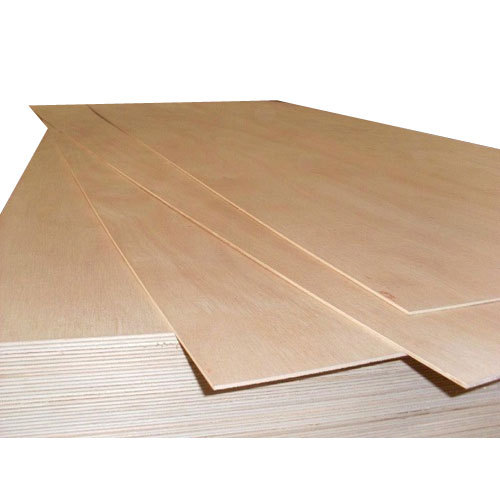
\includegraphics[width=\textwidth]{images/contreplaquet.jpg}
        \caption{Contreplaqué haute densité}
        \label{fig:annexe_contreplaqué}
    \end{minipage}
    \hfill
    \begin{minipage}[b]{0.31\textwidth}
        \centering
        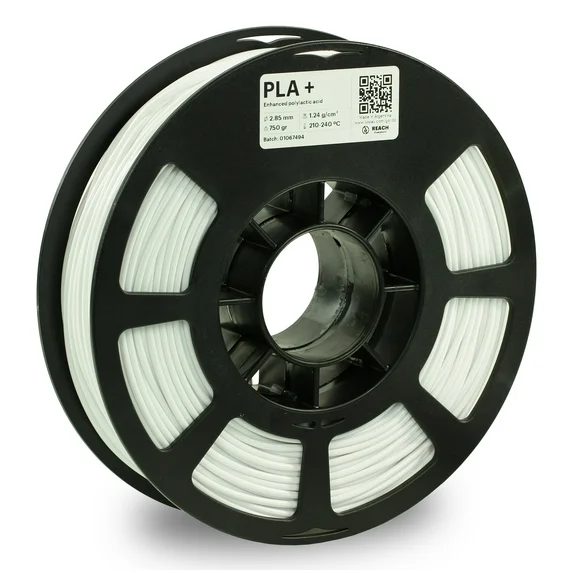
\includegraphics[width=\textwidth]{images/photo-rouleau-pla.png}
        \caption{Filament PLA (impression 3D)}
        \label{fig:annexe_pla}
    \end{minipage}
    \vspace{0.3cm}
    \caption{Matériaux de construction mécanique du châssis SMART-SOJA}
    \label{fig:annexe_materiaux_global}
\end{figure}

\newpage
\cleardoublepage
\stepcounter{chapter}
\chapter*{Annexe \thechapter{} : Schéma électronique global}
\label{annexe:schema_global}
\addcontentsline{toc}{section}{Annexe \thechapter{} : Schéma électronique global}
\setcounter{figure}{0}



Cette annexe présente le schéma électronique global du système SMART-SOJA (Figure \ref{fig:annexe_circuit_global}), regroupant l'ensemble des blocs fonctionnels (alimentation, traitement, puissance, acquisition et IHM) tels que conçus sous KiCad.

\begin{figure}[H]
    \centering
    \includegraphics[width=\textwidth]{images/image_circuit_complet.png}
    \caption{Schéma électronique global du système SMART-SOJA (KiCad)}
    \label{fig:annexe_circuit_global}
\end{figure}

\newpage
\cleardoublepage
\stepcounter{chapter}
\chapter*{Annexe \thechapter{} : Vues détaillées du routage PCB}
\label{annexe:routage_pcb}
\addcontentsline{toc}{section}{Annexe \thechapter{} : Vues détaillées du routage PCB}
\setcounter{figure}{0}



Cette annexe présente les vues de routage des pistes des deux circuits imprimés, comparant la conception sous KiCad (Figures \ref{fig:annexe_pcb_routage_puissance} et \ref{fig:annexe_pcb_routage_commande}) aux circuits imprimés réels après fabrication (Figures \ref{fig:annexe_pcb_routage_puissance_reel} et \ref{fig:annexe_pcb_routage_commande_reel}).

\begin{figure}[H]
    \centering
    \begin{subfigure}[b]{0.48\textwidth}
        \centering
        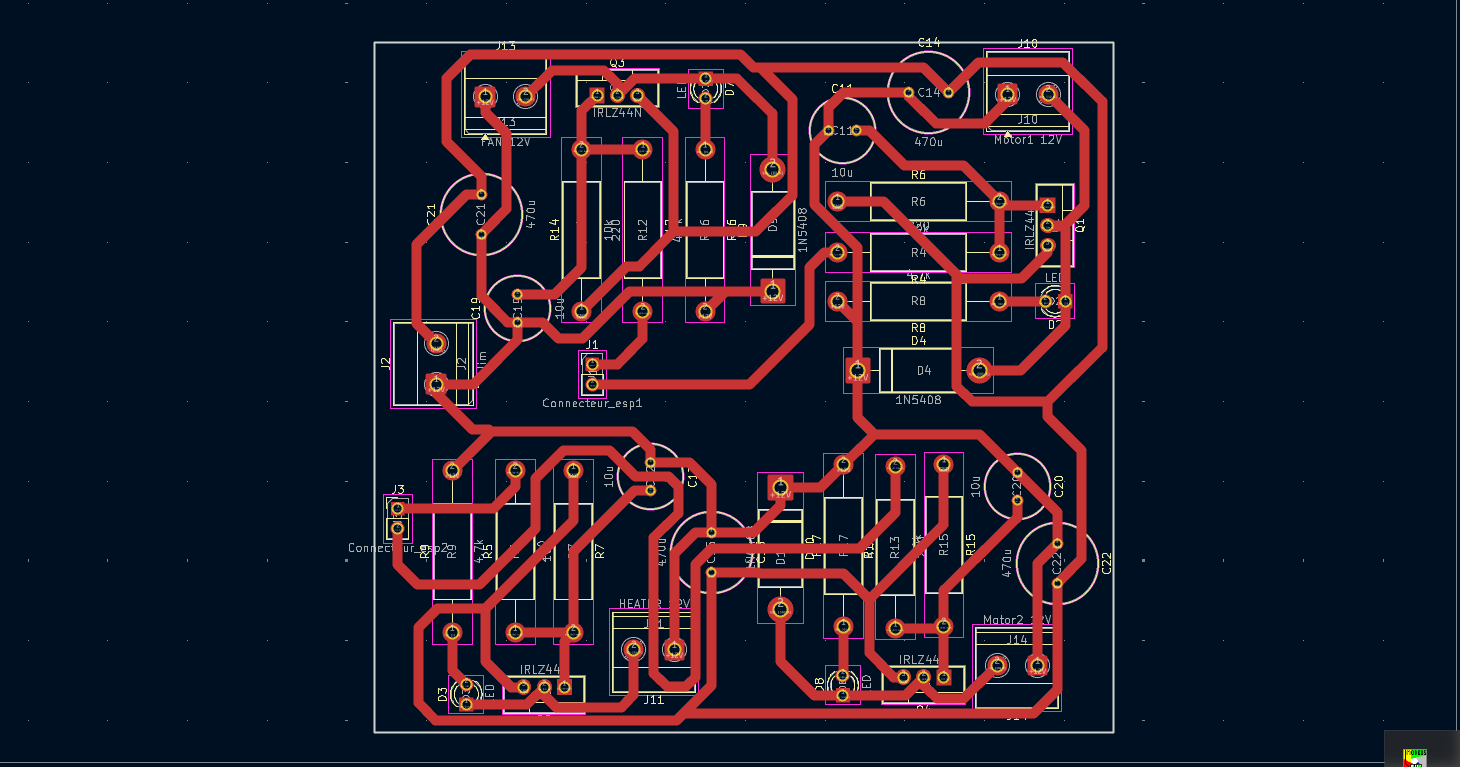
\includegraphics[width=\textwidth]{images/routage_circuit_puissance.png}
        \caption{Conception du routage — Carte puissance}
        \label{fig:annexe_pcb_routage_puissance}
    \end{subfigure}
    \hfill
    \begin{subfigure}[b]{0.48\textwidth}
        \centering
        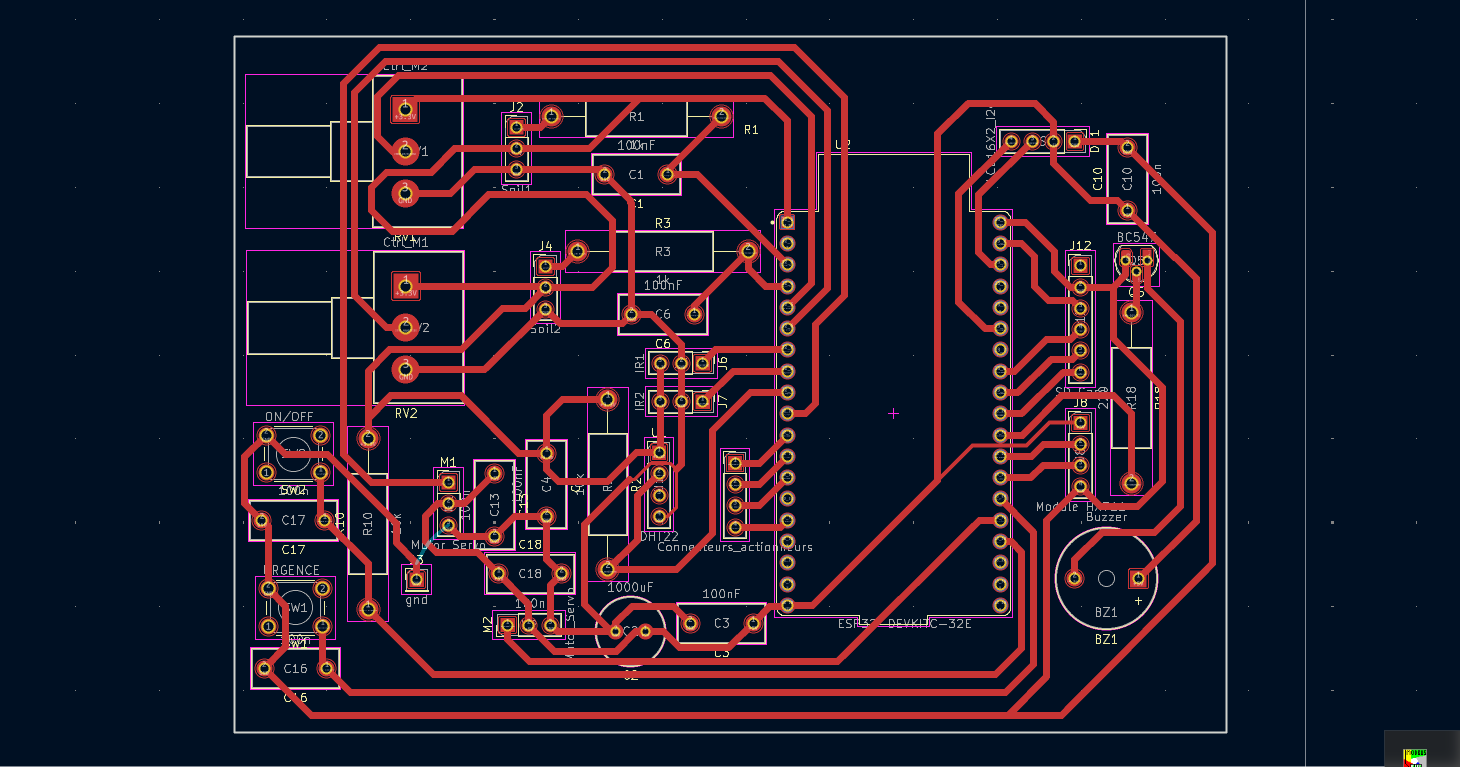
\includegraphics[width=\textwidth]{images/routage_cricuit_commande.png}
        \caption{Conception du routage — Carte commande}
        \label{fig:annexe_pcb_routage_commande}
    \end{subfigure}
    \vspace{0.3cm}
    \begin{subfigure}[b]{0.48\textwidth}
        \centering
        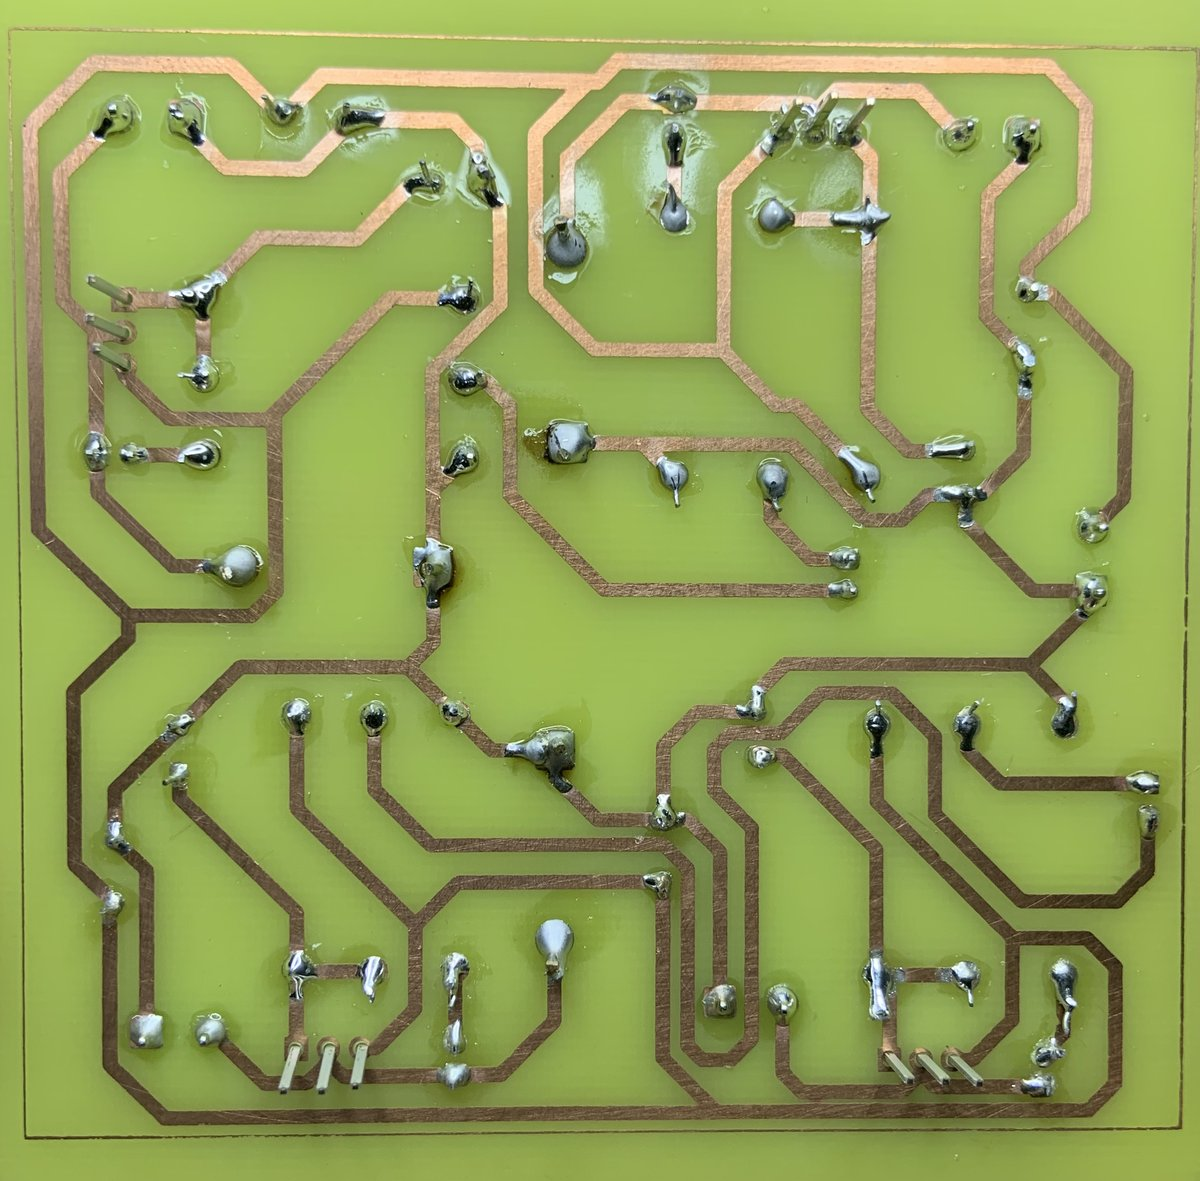
\includegraphics[width=\textwidth]{images/routageReel_circuit_puissance.jpg}
        \caption{Routage réel — Carte puissance}
        \label{fig:annexe_pcb_routage_puissance_reel}
    \end{subfigure}
    \hfill
    \begin{subfigure}[b]{0.48\textwidth}
        \centering
        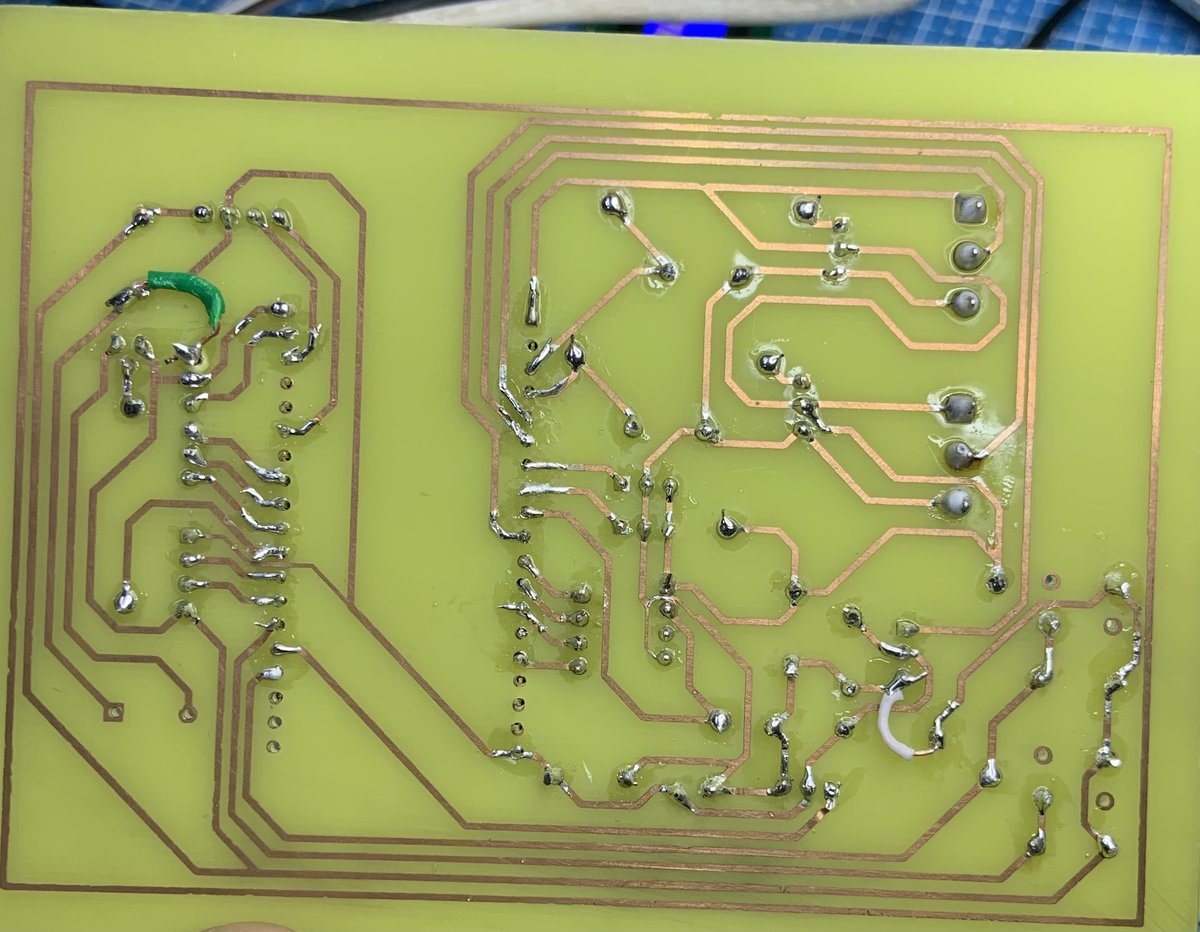
\includegraphics[width=\textwidth]{images/routageReel_circuit_commande.jpg}
        \caption{Routage réel — Carte commande}
        \label{fig:annexe_pcb_routage_commande_reel}
    \end{subfigure}
    \caption{Vues détaillées du routage PCB SMART-SOJA (Conception vs Réel)}
    \label{fig:annexe_pcb_routage}
\end{figure}

\newpage
\cleardoublepage
\stepcounter{chapter}
\chapter*{Annexe \thechapter{} : Vues 3D du circuit imprimé}
\label{annexe:vues_3d_pcb}
\addcontentsline{toc}{section}{Annexe \thechapter{} : Vues 3D du circuit imprimé}
\setcounter{figure}{0}



Les rendus 3D prévisionnels des deux PCB générés sous KiCad (Figures \ref{fig:annexe_pcb_3d_puissance} et \ref{fig:annexe_pcb_3d_commande}) sont ici mis en correspondance avec les photographies des cartes réelles fabriquées et assemblées (Figures \ref{fig:annexe_pcb_3d_puissance_reel} et \ref{fig:annexe_pcb_3d_commande_reel}), permettant de valider l'intégration matérielle finale.

\begin{figure}[H]
    \centering
    \begin{subfigure}[b]{0.48\textwidth}
        \centering
        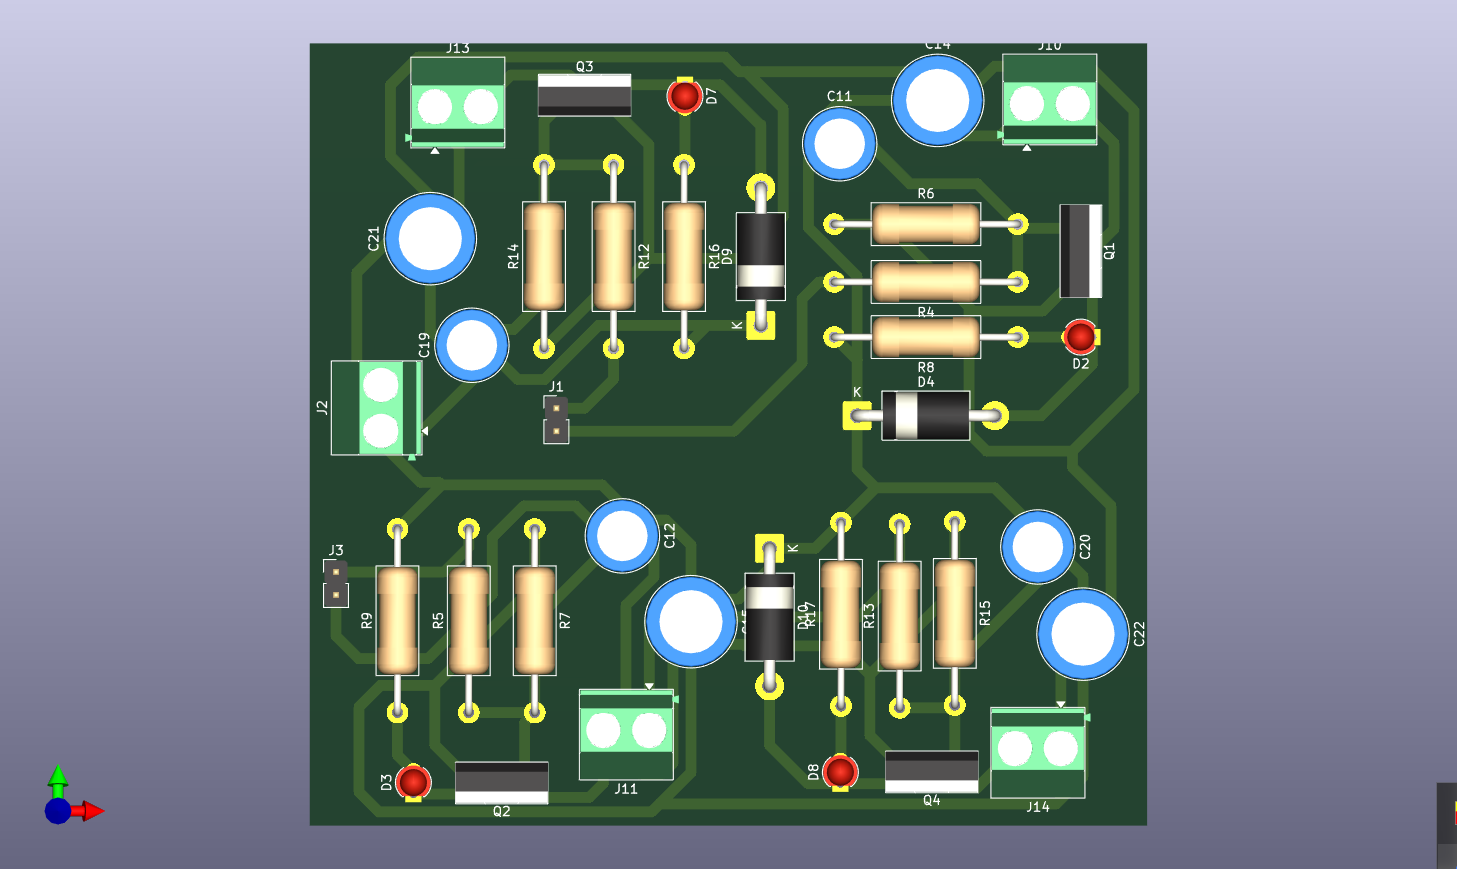
\includegraphics[width=\textwidth]{images/model3D_circuit_puissance.png}
        \caption{Modélisation 3D — Carte puissance}
        \label{fig:annexe_pcb_3d_puissance}
    \end{subfigure}
    \hfill
    \begin{subfigure}[b]{0.48\textwidth}
        \centering
        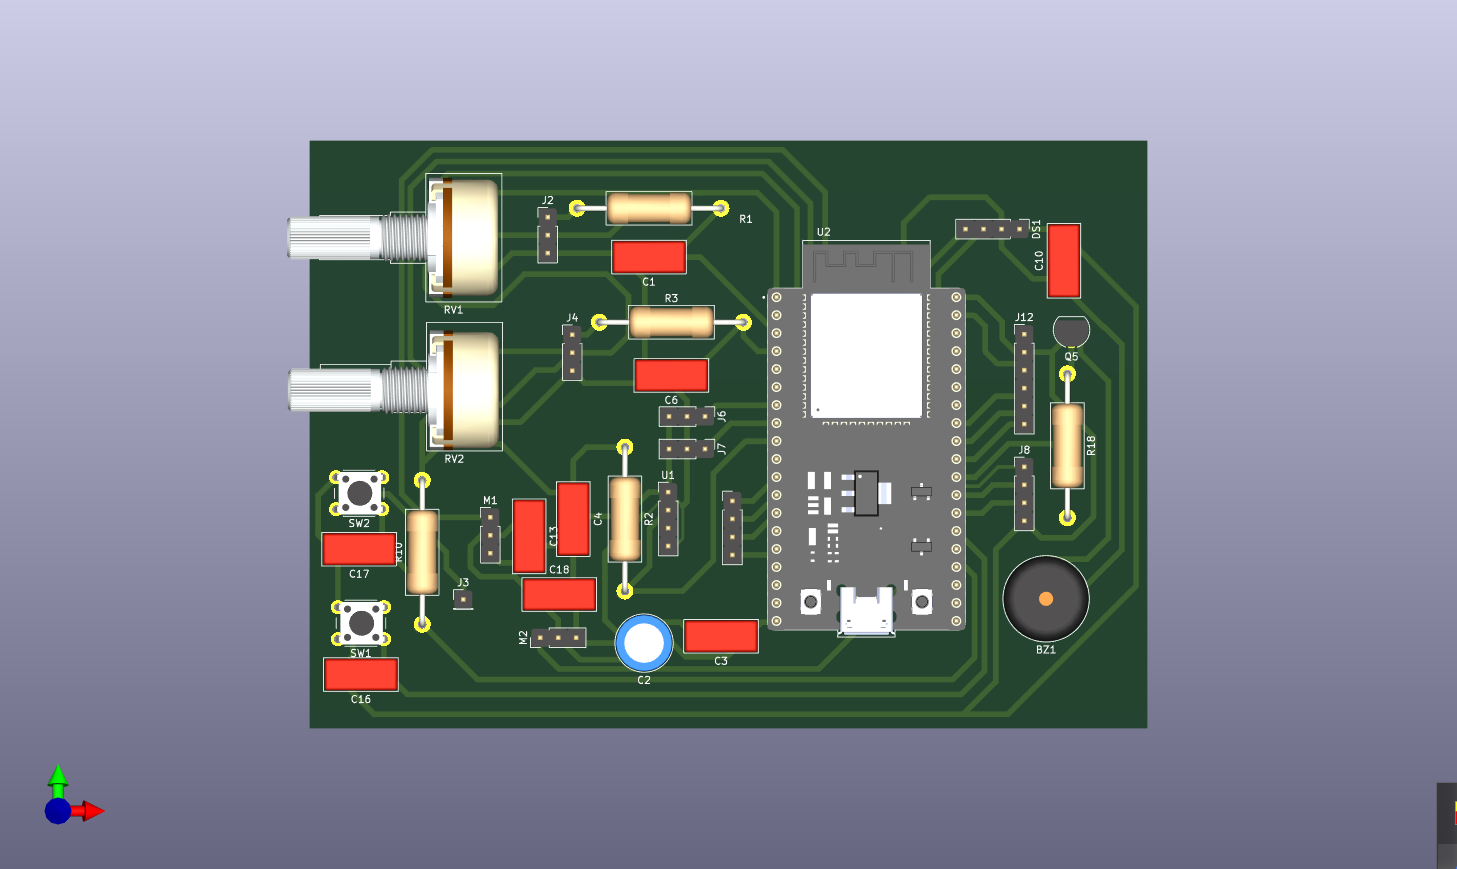
\includegraphics[width=\textwidth]{images/model3D_circuit_commande.png}
        \caption{Modélisation 3D — Carte commande}
        \label{fig:annexe_pcb_3d_commande}
    \end{subfigure}
    \vspace{0.3cm}
    \begin{subfigure}[b]{0.48\textwidth}
        \centering
        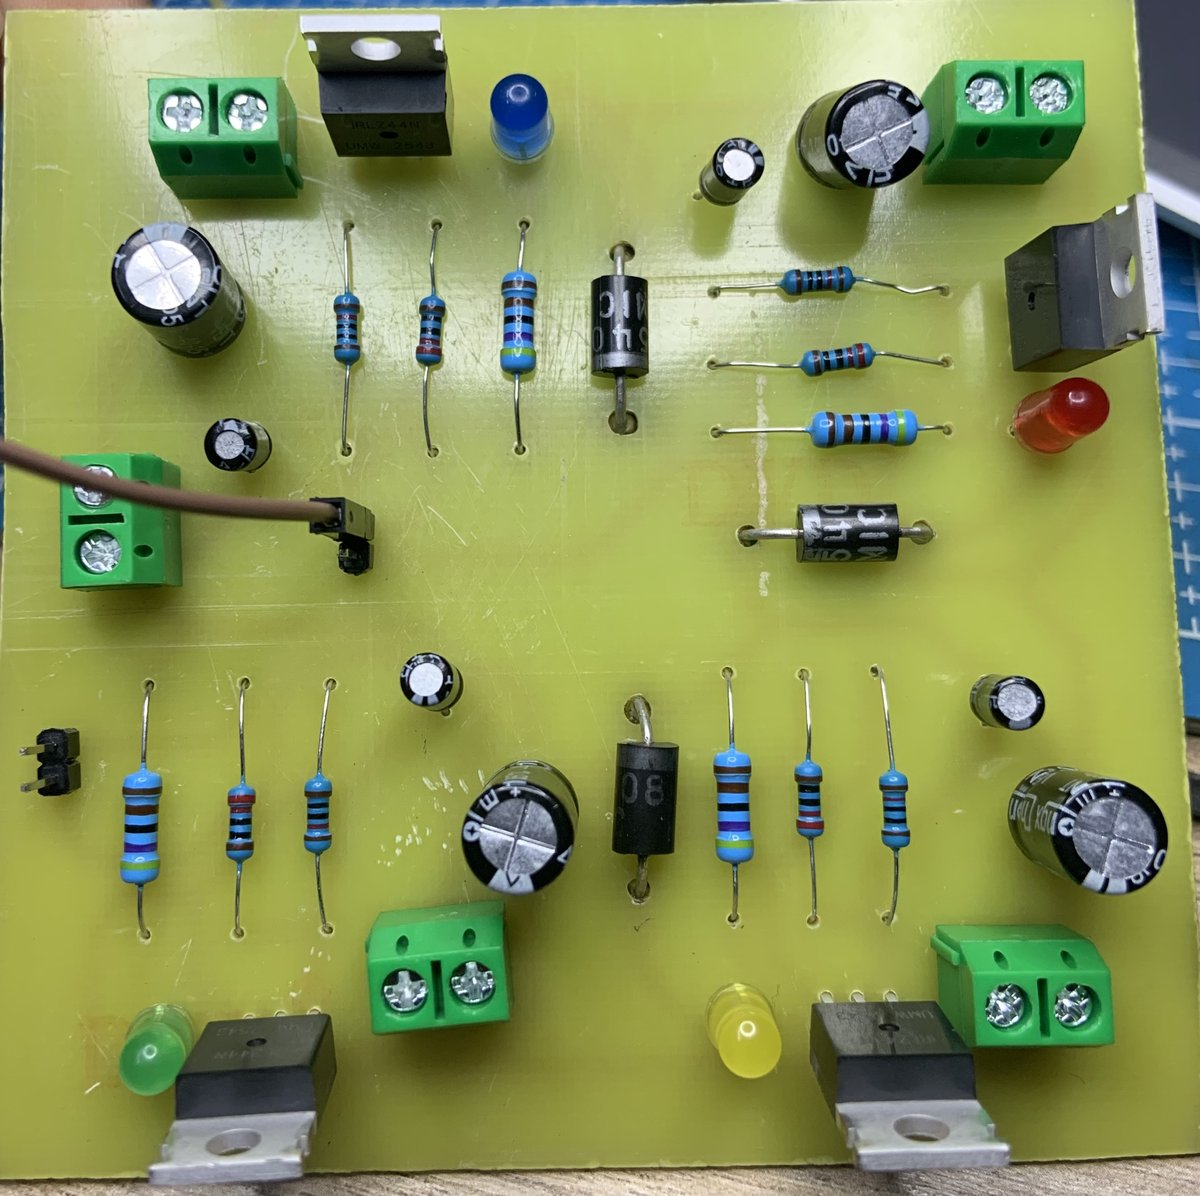
\includegraphics[width=\textwidth]{images/modelReel_circuit_puissance.jpg}
        \caption{Carte puissance réelle (assemblée)}
        \label{fig:annexe_pcb_3d_puissance_reel}
    \end{subfigure}
    \hfill
    \begin{subfigure}[b]{0.48\textwidth}
        \centering
        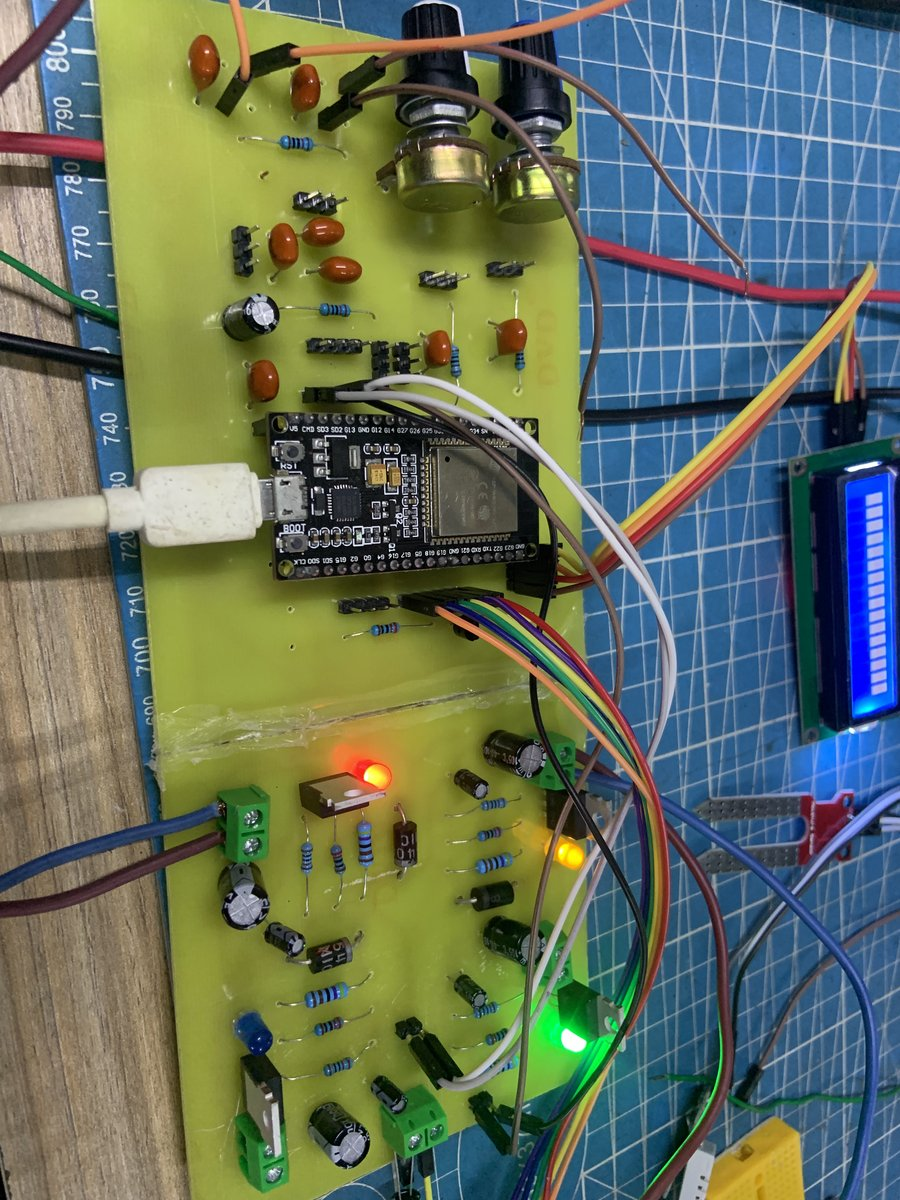
\includegraphics[width=\textwidth]{images/modelReel_circuit_commande.jpg}
        \caption{Carte commande réelle (assemblée)}
        \label{fig:annexe_pcb_3d_commande_reel}
    \end{subfigure}
    \caption{Rendus 3D et cartes réelles assemblées des PCB SMART-SOJA}
    \label{fig:annexe_pcb_3d}
\end{figure}

\newpage
\cleardoublepage
\stepcounter{chapter}
\chapter*{Annexe \thechapter{} : Synoptique de l'alimentation électrique}
\label{annexe:schema_alim}
\addcontentsline{toc}{section}{Annexe \thechapter{} : Synoptique de l'alimentation électrique}
\setcounter{figure}{0}



Cette annexe illustre la chaîne de puissance photovoltaïque du système SMART-SOJA (Figure \ref{fig:annexe_alim_solaire}). Le contrôleur \textbf{SHS 200} de Qotto intègre nativement un \textbf{BMS} (Battery Management System) qui assure la gestion de charge, la protection contre les surcharges et intègre la régulation \textbf{MPPT} pour maximiser l'énergie captée par le panneau solaire. Le bus 12~V alimente directement les charges de puissance (moteurs, ventilateur, résistance chauffante), tandis que les convertisseurs Buck LM2596 abaissent la tension à 5~V pour alimenter l'ESP32 et les capteurs.

\begin{figure}[H]
    \centering
    \resizebox{\textwidth}{!}{
    \begin{tikzpicture}[
        node distance=1.2cm and 1.5cm,
        block/.style={rectangle, draw=ucaoBlue, fill=ucaoBlue!5, text width=6.5em, text centered, rounded corners, minimum height=3em, line width=0.8pt, font=\scriptsize\bfseries},
        arrow/.style={-{Stealth}, line width=1pt, draw=ucaoBlue},
        biarrow/.style={{Stealth}-{Stealth}, line width=1pt, draw=ucaoBlue}
    ]
        % Nodes
        \node (panel)      [block]                      {Panneau\\50~W / 18~V};
        \node (controller) [block, right=of panel]      {SHS 200\\BMS + MPPT};
        \node (battery)    [block, below=of controller] {EV12-20\\12~V / 20~Ah};
        \node (buck)       [block, right=of controller] {LM2596\\12~V $\to$ 5~V};
        \node (loads12)    [block, above right=0.6cm and 1.2cm of controller]
                           {12~V — Puissance\\Moteurs, Ventil., Résist.};
        \node (loads5)     [block, right=of buck]       {5~V — Commande\\ESP32 + Capteurs};

        % Paths
        \draw [arrow]   (panel)      -- node[above, font=\tiny] {18~V DC}  (controller);
        \draw [biarrow] (controller) -- node[right, font=\tiny] {Charge/Décharge} (battery);
        \draw [arrow]   (controller) -- node[above, font=\tiny] {12~V DC}  (loads12);
        \draw [arrow]   (controller) -- node[above, font=\tiny] {12~V DC}  (buck);
        \draw [arrow]   (buck)       -- node[above, font=\tiny] {5~V DC}   (loads5);
    \end{tikzpicture}
    }
    \caption{Synoptique de la chaîne de puissance photovoltaïque SMART-SOJA}
    \label{fig:annexe_alim_solaire}
\end{figure}

